\documentclass{standalone}
\usepackage{tikz}

\usetikzlibrary{calc,math}


\begin{document}

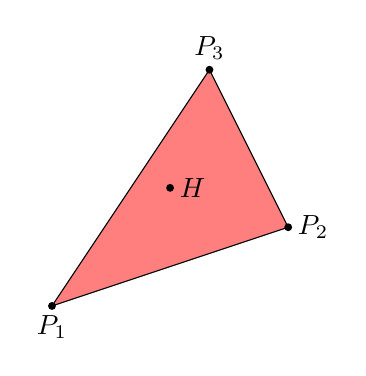
\begin{tikzpicture}
  \coordinate (P1) at (0,0);
  \coordinate (P2) at (3,1);
  \coordinate (P3) at (2,3);
  \coordinate (H) at (1.5,1.5);

  \path[fill=red,opacity=0.5] (P1) -- (P2) -- (P3) -- cycle;
  \draw (P1) -- (P2) -- (P3) -- cycle;

  \path[fill=black] (P1) circle [radius=0.05] node[below] {$P_1$};
  \path[fill=black] (P2) circle [radius=0.05] node[right] {$P_2$};
  \path[fill=black] (P3) circle [radius=0.05] node[above] {$P_3$};
  \path[fill=black] (H) circle [radius=0.05] node[right] {$H$};
\end{tikzpicture}

\end{document}